\documentclass[11pt]{article}
\usepackage[utf8]{inputenc}
%\usepackage[T1]{fontenc}
\usepackage{amssymb}
\usepackage{amsmath}
\usepackage{enumerate}
\usepackage{fullpage}
\usepackage{polski}  
\usepackage{indentfirst} 
\usepackage[pdftex]{graphicx}
\usepackage{multirow}
\usepackage{placeins}

\author{Łukasz Dubiel}
\title{Konspekt}

\begin{document}

\maketitle

\section{Rownanie fali elektormagnetyczne}
$$ \frac{\partial^2 E}{\partial x^2} - \frac{1}{\mu \epsilon} E = 0 $$

$$ \frac{\partial^2 B}{\partial x^2} - \frac{1}{\mu \epsilon} B = 0 $$

\section{Równania maxwella}
$$ \nabla \circ B = 0 $$
$$ \nabla \circ E = \frac{\rho}{\epsilon} $$
$$ \nabla \times E = - \frac{\partial B}{\partial t} $$
$$ \nabla \times B = \mu j - \mu \epsilon \frac{\partial E}{\partial t} $$

\section{Dyfrakcja i interferencja}
Interferencja - zjawisko powstawania przestrzennego rozkładu amplitud w wyniku superpozycji dwóch fal.

Dyfrakcja - zmiana kierunku rozchodzenia się fali na krawędziach.

\section{Analogia do fali do sprężystych}

...

\section{Obraz dyfrakcyjny}
Obraz na rzutni po przejściu wiązki światła przez siatkę dyfrakcyjną.
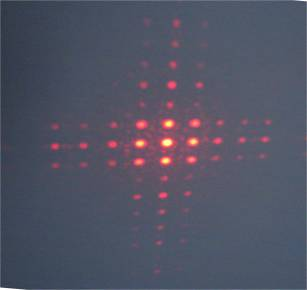
\includegraphics{image018.jpg}

\section{Inne elementy fyfrakcyjne}
Płyty CD

\section{Rodzaje polaryzacji}
\begin{enumerate}
\item{Liniowa}
\item{Kołowa}
\item{Eliptyczna}
\end{enumerate}

\begin{enumerate}
\item{Lewoskrętnie}
\item{Prawoskrętnie}
\end{enumerate}

\ section{Sposoby uzyskiwania światła spolaryzowanego}
\begin{enumerate}
\item{Przepuszczenie przez kryształ dwójłomny}
\item{Odbicie}
\item{Polaryzotory}
\item{Selektywne pochłanianie}
\end{enumerate}
\section{Polaryzatory}
\begin{enumerate}
\item{Polaroid}
\item{Odbiciowy}
\end{enumerate}

\section{Prawo malusa}
$$ I = I_0 \cos^2{\varphi} $$



\end{document}
